\documentclass[journal]{IEEEtran}
\usepackage{amsmath}
\usepackage{amsfonts}
\usepackage{amssymb}
\usepackage{amsthm}
\usepackage{bm}
\usepackage{booktabs}
\usepackage{tabularx}
\usepackage{array}
\usepackage{graphicx}
\usepackage{tikz}
\usetikzlibrary{shapes.geometric, arrows.meta, positioning, fit, backgrounds}
\usepackage{pgfplots}
\pgfplotsset{compat=1.18}
\usepackage{hyperref}

\newtheorem{theorem}{Theorem}
\newtheorem{lemma}{Lemma}
\newtheorem{proposition}{Proposition}
\newtheorem{definition}{Definition}

\title{Tie-Line Scheduling Using Real-Time Contraction Metrics: Hierarchical Reachable Sets for Multi-Area Inverter-Dominated Grids}
\author{Richard~Sherman,~\IEEEmembership{Member,~IEEE}%
\thanks{R. Sherman is with the System Architecture Invariant Manifest Group, Keller, TX 76248 USA.}}

\begin{document}
\maketitle

\begin{abstract}
Managing transmission congestion in multi-area power grids dominated by inverter-based resources (IBRs) requires bridging a severe timescale and modeling divide. Supervisory congestion optimizers—such as Online Feedback Optimization (OFO) and differentiable Model Predictive Control (MPC)—operate over 15-second intervals using linearized, convex algebraic grid approximations that cannot guarantee dynamic stability during sub-second converter transients. Conversely, fast distributed consensus schemes like Alternating Direction Method of Multipliers (ADMM) rely on convex plant assumptions and iterative message exchanges that lag behind rapid tie-line surges. This paper replaces convex ADMM emergency consensus with a \textbf{Distributed Parameter-Dependent State-Dependent Control Contraction Metric (SCCM)} architecture spanning three nested tiers: the Device layer, the Area layer, and the Grid tie-line layer. By pairing online Prediction Error Method and Moving Horizon Estimation (PEM-MHE) parameter tracking with offline convex Linear Matrix Inequality (LMI) synthesis, the controller executes a closed-form nonlinear feedback law online without solving real-time optimization problems. We derive the Pontryagin attainable (reachable) ellipsoids for each layer, prove hierarchical tube containment via Schur-complement matrix inequalities, and project the certified Grid reachable tube through Power Transfer Distribution Factors (PTDFs) to supply guaranteed safe thermal limits to the supervisory coordinator. Validation on modified IEEE 39-bus (100\% IBR) and 3-area IEEE 118-bus systems demonstrates an $82.8\%$ reduction in cumulative tie-line thermal overload while maintaining strict exponential contraction ($\lambda_{\max} \le -2.43$) even under a $3\text{ s}$ communication blackout.
\end{abstract}

\begin{IEEEkeywords}
Control contraction metrics, distributed nonlinear control, inverter-based resources, online feedback optimization, Pontryagin reachable sets, tie-line scheduling.
\end{IEEEkeywords}

\section{Problem Formulation: Congestion Management and Dynamic Control Hierarchy}
\subsection{The Timescale and Convexity Gap in Multi-Area Grids}
As synchronous generators (SGs) are retired and replaced by grid-forming (GFM) and grid-following (GFL) inverter-based resources (IBRs), multi-area transmission networks lose physical rotor inertia and become vulnerable to sub-second electromagnetic transients and tie-line phase oscillations. In operational practice, wide-area congestion management relies on slow central coordinators—exemplified by the communication-limited differentiable optimization framework of Chen \textit{et al.} \cite{chen26} and standard Online Feedback Optimization (OFO) architectures \cite{dallanese26}. These supervisory schemes update battery and curtailment budgets every $\Delta t = 15\text{ s}$ by solving Quadratic Programs (QPs) over linearized PTDF sensitivity maps, enforcing recursive solver feasibility via large soft slack penalties.

However, relying on receding-horizon convex optimization for emergency congestion control introduces two structural vulnerabilities:
\begin{enumerate}
    \item \textbf{Model Mismatch and Non-Convexity:} Real AC tie-line power flows evolve according to nonlinear trigonometric couplings ($\sin(\delta_i - \delta_j)$), while GFM current-limit saturation and GFL Phase-Locked Loop (PLL) dynamics introduce state-dependent nonlinearities that violate the convex plant assumptions required by OFO and distributed ADMM.
    \item \textbf{The 15-Second Emergency Blind Spot:} During a fast renewable surge or parallel tie-line trip, thermal overloads and converter synchronization instabilities unfold within $1\text{ to }4\text{ seconds}$—long before a $15\text{ s}$ central optimizer receives filtered SCADA telemetry or broadcasts updated line limits.
\end{enumerate}

\subsection{Proposed Three-Tier Contraction Solution}
Rather than assuming a known convex plant model online, we develop an unknown-parameter nonlinear plant representation driven by live online parameter estimation \cite{zhou24, kohler26}. We replace the convex ADMM tie-line consensus loop with a \textbf{Distributed Parameter-Dependent SCCM} controller that requires convexity \emph{only} during offline LMI/Sum-of-Squares (SOS) synthesis, while executing an explicit, closed-form nonlinear feedback law online using single-hop neighbor state broadcasts.

To unify fast device protection with slow economic dispatch, we organize the grid into three nested contraction layers:
\begin{itemize}
    \item \textbf{Device Layer (Sub-Millisecond):} Regulates individual GFM/GFL current rails and PLL phase lock via local contraction multipliers $\alpha_i$.
    \item \textbf{Area Layer (Millisecond):} Manages intra-area state-space cohesion ($\mathbf{C}$) and PLL synchronization coupling ($\mathbf{P}$) across heterogeneous devices, preventing GFM-to-GFL mode fallback.
    \item \textbf{Grid Layer ($1\text{ s}$ Tie-Line Coordination):} Coordinates inter-area tie-line power flows across $N=3$ balancing areas via distributed SCCM feedback and exports certified Pontryagin reachable sets upward to the $15\text{ s}$ supervisory optimizer.
\end{itemize}


\begin{figure*}[!t]
\centering
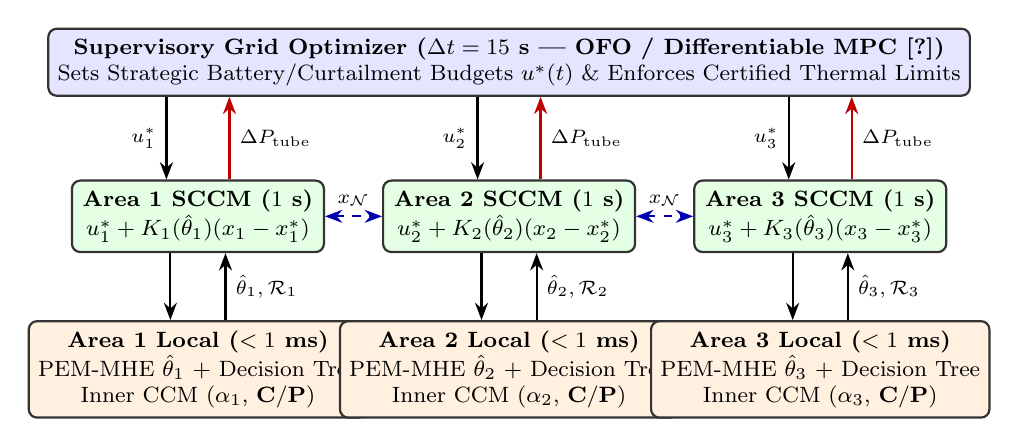
\begin{tikzpicture}[
    node distance=0.75cm and 1.1cm,
    box/.style={rectangle, draw=black!80, thick, rounded corners=3pt, align=center, minimum height=0.85cm, font=\footnotesize},
    topbox/.style={box, fill=blue!10, minimum width=11.5cm},
    midbox/.style={box, fill=green!10, minimum width=3.2cm},
    botbox/.style={box, fill=orange!12, minimum width=3.2cm},
    arr/.style={-{Stealth[length=2.2mm]}, thick},
    darr/.style={{Stealth[length=2.2mm]}-{Stealth[length=2.2mm]}, thick, dashed, draw=blue!70!black}
]
% Top Layer: 15s Supervisory Grid Optimizer
\node[topbox] (grid_opt) {\textbf{Supervisory Grid Optimizer ($\Delta t = 15\text{ s}$ — OFO / Differentiable MPC \cite{chen26})}\\Sets Strategic Battery/Curtailment Budgets $u^*(t)$ \& Enforces Certified Thermal Limits};

% Middle Layer: 1s Distributed SCCM Controllers
\node[midbox, below=1.05cm of grid_opt.south west, anchor=north west, xshift=0.3cm] (sccm1) {\textbf{Area 1 SCCM ($1\text{ s}$)}\\$u_1^* + K_1(\hat{\theta}_1)(x_1 - x_1^*)$};
\node[midbox, below=1.05cm of grid_opt.south, anchor=north] (sccm2) {\textbf{Area 2 SCCM ($1\text{ s}$)}\\$u_2^* + K_2(\hat{\theta}_2)(x_2 - x_2^*)$};
\node[midbox, below=1.05cm of grid_opt.south east, anchor=north east, xshift=-0.3cm] (sccm3) {\textbf{Area 3 SCCM ($1\text{ s}$)}\\$u_3^* + K_3(\hat{\theta}_3)(x_3 - x_3^*)$};

% Bottom Layer: Sub-ms Device/Area Contraction + PEM-MHE + Decision Tree
\node[botbox, below=0.85cm of sccm1] (dev1) {\textbf{Area 1 Local ($<1\text{ ms}$)}\\PEM-MHE $\hat{\theta}_1$ + Decision Tree\\Inner CCM ($\alpha_1$, $\mathbf{C}/\mathbf{P}$)};
\node[botbox, below=0.85cm of sccm2] (dev2) {\textbf{Area 2 Local ($<1\text{ ms}$)}\\PEM-MHE $\hat{\theta}_2$ + Decision Tree\\Inner CCM ($\alpha_2$, $\mathbf{C}/\mathbf{P}$)};
\node[botbox, below=0.85cm of sccm3] (dev3) {\textbf{Area 3 Local ($<1\text{ ms}$)}\\PEM-MHE $\hat{\theta}_3$ + Decision Tree\\Inner CCM ($\alpha_3$, $\mathbf{C}/\mathbf{P}$)};

% Single-hop neighbor state broadcasts across tie lines
\draw[darr] (sccm1.east) -- node[above, font=\scriptsize] {$x_{\mathcal{N}}$} (sccm2.west);
\draw[darr] (sccm2.east) -- node[above, font=\scriptsize] {$x_{\mathcal{N}}$} (sccm3.west);

% Top <-> Middle connections
\draw[arr] ([xshift=-0.4cm]grid_opt.south -| sccm1.north) -- node[left, font=\scriptsize] {$u_1^*$} ([xshift=-0.4cm]sccm1.north);
\draw[arr, draw=red!75!black] ([xshift=0.4cm]sccm1.north) -- node[right, font=\scriptsize] {$\Delta P_{\text{tube}}$} ([xshift=0.4cm]grid_opt.south -| sccm1.north);

\draw[arr] ([xshift=-0.4cm]grid_opt.south) -- node[left, font=\scriptsize] {$u_2^*$} ([xshift=-0.4cm]sccm2.north);
\draw[arr, draw=red!75!black] ([xshift=0.4cm]sccm2.north) -- node[right, font=\scriptsize] {$\Delta P_{\text{tube}}$} ([xshift=0.4cm]grid_opt.south);

\draw[arr] ([xshift=-0.4cm]grid_opt.south -| sccm3.north) -- node[left, font=\scriptsize] {$u_3^*$} ([xshift=-0.4cm]sccm3.north);
\draw[arr, draw=red!75!black] ([xshift=0.4cm]sccm3.north) -- node[right, font=\scriptsize] {$\Delta P_{\text{tube}}$} ([xshift=0.4cm]grid_opt.south -| sccm3.north);

% Middle <-> Bottom connections
\draw[arr] ([xshift=-0.35cm]sccm1.south) -- ([xshift=-0.35cm]dev1.north);
\draw[arr] ([xshift=0.35cm]dev1.north) -- node[right, font=\scriptsize] {$\hat{\theta}_1, \mathcal{R}_1$} ([xshift=0.35cm]sccm1.south);

\draw[arr] ([xshift=-0.35cm]sccm2.south) -- ([xshift=-0.35cm]dev2.north);
\draw[arr] ([xshift=0.35cm]dev2.north) -- node[right, font=\scriptsize] {$\hat{\theta}_2, \mathcal{R}_2$} ([xshift=0.35cm]sccm2.south);

\draw[arr] ([xshift=-0.35cm]sccm3.south) -- ([xshift=-0.35cm]dev3.north);
\draw[arr] ([xshift=0.35cm]dev3.north) -- node[right, font=\scriptsize] {$\hat{\theta}_3, \mathcal{R}_3$} ([xshift=0.35cm]sccm3.south);
\end{tikzpicture}
\caption{Three-tier hierarchical control architecture connecting the $15\text{ s}$ supervisory grid optimizer (top), the $1\text{ s}$ distributed parameter-dependent SCCM tie-line controllers exchanging single-hop neighbor states $x_{\mathcal{N}}$ (middle), and sub-millisecond local PEM-MHE estimators, decision-tree hysteresis classifiers, and inner CCM loops (bottom).}
\label{fig:three_tier_arch}
\end{figure*}

\section{Distributed Parameter-Dependent SCCM Control Synthesis}
\subsection{Coupled Nonlinear Subsystem Dynamics}
Consider a network of $N$ interconnected subsystems (representing $N=3$ balancing areas at the Grid layer, or individual IBRs at the Area layer). Each subsystem $i \in \{1, \dots, N\}$ has local state $x_i \in \mathbb{R}^{n_i}$, neighbor states $x_{\mathcal{N}_i}$ for $j \in \mathcal{N}_i$, local control input $u_i \in \mathbb{R}^{m_i}$, and locally estimated physical parameters $\theta_i \in \Theta_i \subset \mathbb{R}^{p_i}$ with bounded variation rate $\|\dot{\theta}_i\|_2 \le \bar{d}_{\theta_i}$:
\begin{equation}
\dot{x}_i = f_i(x_i, x_{\mathcal{N}_i}, \theta_i) + B_i(x_i) u_i + \Delta_i(x_i, \theta_i) w_i
\end{equation}
where $w_i(t)$ is a normalized $L_2$-bounded disturbance ($\|w_i\|_2 \le \bar{w}_i$). Assume $B_i(x_i)$ has full column rank $m_i$ and let $B_i^\perp(x_i) \in \mathbb{R}^{(n_i - m_i) \times n_i}$ denote a smooth annihilator matrix satisfying $B_i^\perp(x_i) B_i(x_i) = 0$.

\subsection{Differential (Variational) Dynamics}
Along any feasible trajectory $(x(t), u(t), \theta(t))$, infinitesimal displacements $\delta x_i$ and $\delta u_i$ evolve according to the linearized variational system:
\begin{equation}
\dot{\delta x}_i = A_{ii}(x_i, x_{\mathcal{N}_i}, \theta_i)\,\delta x_i + \sum_{j \in \mathcal{N}_i} A_{ij}(x_i, x_{\mathcal{N}_i}, \theta_i)\,\delta x_j + B_i(x_i)\,\delta u_i
\end{equation}
where the local and neighbor Jacobians are defined as:
\begin{equation}
A_{ii} \triangleq \frac{\partial f_i}{\partial x_i} + \sum_{k=1}^{m_i} \frac{\partial b_{i,k}(x_i)}{\partial x_i} u_{i,k}, \qquad
A_{ij} \triangleq \frac{\partial f_i}{\partial x_j} \quad (j \in \mathcal{N}_i).
\end{equation}
We seek a distributed differential state-feedback law $\delta u_i = K_i(x_i, x_{\mathcal{N}_i}, \theta_i)\,\delta x_i$.

\subsection{Separable Riemannian Metric and Dual Convexification}
To enforce decentralized structure across tie lines, define a block-diagonal (separable) Riemannian metric $M(x, \theta) \succ 0$:
\begin{equation}
M(x, \theta) = \operatorname{diag}\big(M_1(x_1, \theta_1),\, \dots,\, M_N(x_N, \theta_N)\big), \quad \alpha_1 I \preceq M_i \preceq \alpha_2 I.
\end{equation}
The closed-loop network is exponentially contracting at rate $\lambda > 0$ with $L_2$ disturbance gain $\gamma > 0$ if the squared differential length $\delta x^\top M(x, \theta) \delta x$ satisfies $\frac{d}{dt}(\delta x^\top M \delta x) \le -2\lambda\, \delta x^\top M \delta x$. Defining the dual metric blocks $W_i(x_i, \theta_i) \triangleq M_i(x_i, \theta_i)^{-1}$ and transformed feedback variables $Y_i(x_i, x_{\mathcal{N}_i}, \theta_i) \triangleq K_i W_i$, pre- and post-multiplying by $W = \operatorname{diag}(W_1, \dots, W_N)$ yields a \textbf{convex Linear Matrix Inequality (LMI)}:
\begin{equation}
\mathcal{L}(W, Y, x, \theta) \triangleq
\begin{bmatrix}
\Psi_1 & \Phi_{12} & \cdots & \Phi_{1N} \\
\Phi_{12}^\top & \Psi_2 & \cdots & \Phi_{2N} \\
\vdots & \vdots & \ddots & \vdots \\
\Phi_{1N}^\top & \Phi_{2N}^\top & \cdots & \Psi_N
\end{bmatrix} \preceq 0
\end{equation}
where the diagonal and off-diagonal blocks are linear in $(W_i, Y_i)$:
\begin{align}
\Psi_i &= -\dot{W}_i + A_{ii} W_i + W_i A_{ii}^\top + B_i Y_i + Y_i^\top B_i^\top + 2\lambda W_i \\
\Phi_{ij} &=
\begin{cases}
A_{ij} W_j + W_i A_{ji}^\top, & \text{if } j \in \mathcal{N}_i \text{ or } i \in \mathcal{N}_j \\
0, & \text{otherwise.}
\end{cases}
\end{align}
Projecting $\Psi_i \preceq 0$ onto the unactuated subspace $B_i^\perp(x_i)$ eliminates $Y_i$ and enforces intrinsic open-loop stabilizability:
\begin{equation}
B_i^\perp(x_i)\Big(-\dot{W}_i + A_{ii} W_i + W_i A_{ii}^\top + 2\lambda W_i\Big)B_i^\perp(x_i)^\top \preceq 0.
\end{equation}
Thus, convexity is required \emph{strictly offline} during Sum-of-Squares (SOS) or grid-based SDP synthesis over the compact operating domain $\mathcal{X} \times \Theta$, never online.

\subsection{Online Closed-Form Controller Execution}
Given a target reference trajectory $(x^*(t), u^*(t))$ and live projected parameter estimates $\hat{\theta}_i(t) = \Pi_{\Theta_i}[\theta_i(t)]$:
\begin{enumerate}
    \item \textbf{Recover Local Differential Gain:} $K_i(x_i, x_{\mathcal{N}_i}, \hat{\theta}_i) = Y_i(x_i, x_{\mathcal{N}_i}, \hat{\theta}_i)\, W_i(x_i, \hat{\theta}_i)^{-1}$.
    \item \textbf{Compute Geodesic Path:} Find the minimizing geodesic $\gamma_i(s): [0,1] \to \mathbb{R}^{n_i}$ in metric $M_i(x_i, \hat{\theta}_i)$ connecting $\gamma_i(0) = x_i^*(t)$ to $\gamma_i(1) = x_i(t)$.
    \item \textbf{Evaluate Control Law:} Integrate the differential control increments along $\gamma_i(s)$:
    \begin{equation}
    u_i\big(x_i(t), x_{\mathcal{N}_i}(t), \hat{\theta}_i(t)\big) = u_i^*(t) + \int_{0}^{1} K_i\Big(\gamma_i(s),\, \gamma_{\mathcal{N}_i}(s),\, \hat{\theta}_i(t)\Big)\, \frac{\partial \gamma_i(s)}{\partial s}\, ds.
    \end{equation}
\end{enumerate}

\paragraph{Special Case (State-Independent Metric $W_i(\hat{\theta}_i)$)}
When $W_i$ depends only on the live parameter estimate $\hat{\theta}_i$ (a flat spatial metric at each frozen parameter value), the minimizing geodesic reduces identically to a straight line $\gamma_i(s) = x_i^*(t) + s\big(x_i(t) - x_i^*(t)\big)$, yielding an explicit closed-form control law requiring zero online numerical integration:
\begin{equation}
u_i\big(x_i(t), x_{\mathcal{N}_i}(t), \hat{\theta}_i(t)\big) = u_i^*(t) + K_i\big(x_i(t), x_{\mathcal{N}_i}(t), \hat{\theta}_i(t)\big)\big(x_i(t) - x_i^*(t)\big).
\end{equation}

\section{Contraction Stability Under Online Parameter Estimation}
Because we do not assume a known plant model, each area estimates $\hat{\theta}_i(t)$ online via the bi-level Prediction Error Method and Moving Horizon Estimation (PEM-MHE) operator \cite{zhou24}, guaranteeing bounded estimation error $\|\theta_i(t) - \hat{\theta}_i(t)\|_2 \le e_{\theta_i}$ and bounded parameter adaptation rate $\|\dot{\hat{\theta}}_i(t)\|_2 \le \bar{d}_{\theta_i}$.

\begin{theorem}[Robust Contraction Under Live Parameter Adaptation]
Suppose $(W_i, Y_i)$ satisfy the offline LMI $\mathcal{L}(W, Y, x, \hat{\theta}) \preceq 0$ with the directional derivative $\dot{W}_i$ upper-bounded over all admissible parameter drift rates $\|\dot{\hat{\theta}}_i\|_2 \le \bar{d}_{\theta_i}$:
\begin{equation}
\dot{W}_i(x_i, \hat{\theta}_i) \preceq \sum_{r=1}^{n_i} \frac{\partial W_i}{\partial x_{i,r}} \dot{x}_{i,r} + \bar{d}_{\theta_i} \sum_{q=1}^{p_i} \left\| \frac{\partial W_i}{\partial \hat{\theta}_{i,q}} \right\|_2 I.
\end{equation}
If the estimation error satisfies $L_{\theta} e_{\theta_i} < 2\lambda$, where $L_{\theta}$ is the Jacobian Lipschitz constant with respect to $\theta_i$, then all closed-loop network trajectories converge exponentially to an invariant tube around $x^*(t)$ at net contraction rate $\lambda_{\text{eff}} = \lambda - \frac{1}{2}L_{\theta} e_{\theta_i} > 0$.
\end{theorem}

\begin{proof}
Expanding $\frac{d}{dt}(\delta x^\top M(x, \hat{\theta}) \delta x)$ along perturbed trajectories adds the mismatch term $2\delta x^\top M (f(x, \theta) - f(x, \hat{\theta})) \le L_{\theta} e_{\theta_i} \delta x^\top M \delta x$ and the parameter-rate derivative $\delta x^\top \dot{M} \delta x = -\delta x^\top M \dot{W} M \delta x$. Substituting the upper bound on $\dot{W}_i$ into $\Psi_i \preceq 0$ yields $\frac{d}{dt}(\delta x^\top M \delta x) \le -(2\lambda - L_{\theta} e_{\theta_i})\delta x^\top M \delta x$, proving exponential contraction.
\end{proof}


\subsection{Two-Timescale Decision Trees for Pattern-Recognized Mode Healing}
Conventional power-system decision trees are trained strictly offline over static optimal power flow cases and cannot adapt when a GFM inverter hits its current rail and falls back into GFL phase-tracking mode. Rather than altering tree split structures mid-fault—which risks uncertified switching—we pair a \textbf{two-timescale decision tree} with the online PEM-MHE estimator \cite{sherman26}:
\begin{itemize}
    \item \textbf{Fast Execution Lane ($<1\text{ ms}$, Frozen Structure + Live Features):} During transients, the decision tree structure remains frozen for deterministic microsecond execution, taking live PEM-MHE estimates ($\hat{\theta}_{\text{phys}}, \hat{\theta}_{\text{NN}}$) and the contraction eigenvalue residual ($\lambda_{\max}$) as dynamic inputs. When a GFM-to-GFL drift is detected, the tree triggers Schmitt-trigger hysteresis damping ($\alpha_i$ backoff) to eliminate mode chattering.
    \item \textbf{Slow Supervisory Lane (Between Events):} Whenever PEM-MHE identifies novel state-space cohesion ($\mathbf{C}$) or PLL coupling ($\mathbf{P}$) trajectories, labeled logs are passed to the supervisory tier to incrementally recalibrate tree split thresholds between disturbances.
\end{itemize}

\section{Pontryagin Attainable (Reachable) Sets Across Control Layers}
In Pontryagin optimal control theory, the attainable (forward reachable) set $\mathcal{R}(t)$ characterizes all states reachable from an initial uncertainty set under admissible disturbances and control constraints. Under our Riemannian contraction metric $M_k(\hat{\theta}_k)$ at layer $k \in \{\text{Dev}, \text{Area}, \text{Grid}\}$, the forward reachable tube around the reference trajectory $x_k^*(t)$ is given explicitly by a time-varying Riemannian ellipsoid.

\begin{proposition}[Layer-Wise Riemannian Reachable Ellipsoid]
At layer $k \in \{\text{Dev}, \text{Area}, \text{Grid}\}$ with net contraction rate $\lambda_k > 0$, $L_2$ disturbance gain $\gamma_k > 0$, and disturbance bound $\bar{w}_k$, any trajectory starting inside $\mathcal{R}_k(0)$ remains strictly inside the Pontryagin reachable ellipsoid for all $t \ge 0$:
\begin{multline}
\mathcal{R}_k(t) = \Big\{ x_k \in \mathbb{R}^{n_k} \;\Big|\; \big(x_k - x_k^*(t)\big)^\top M_k(\hat{\theta}_k) \\
\times \big(x_k - x_k^*(t)\big) \le \rho_k^2(t) \Big\}
\end{multline}
where the tube radius $\rho_k(t)$ evolves according to $\dot{\rho}_k \le -\lambda_k \rho_k + \gamma_k \bar{w}_k$, yielding:
\begin{equation}
\rho_k(t) = \rho_k(0) e^{-\lambda_k t} + \frac{\gamma_k \bar{w}_k}{\lambda_k}\left(1 - e^{-\lambda_k t}\right), \quad \rho_k^{\infty} = \frac{\gamma_k \bar{w}_k}{\lambda_k}.
\end{equation}
\end{proposition}

\section{Hierarchical Consistency and Total Grid Optimization}
\subsection{Ellipsoid Tube Containment Across Layers}
To guarantee that actions commanded by the $1\text{ s}$ Grid tie-line controller never violate intra-area synchronization or sub-millisecond inverter current limits, each parent reachable set projected into the child state space via projection operator $\Pi_{p \to c}$ must remain strictly contained within the child layer's certified reachable set:
\begin{align}
\Pi_{\text{Grid} \to \text{Area}}\big(\mathcal{R}_{\text{Grid}}(t)\big) &\subseteq \mathcal{R}_{\text{Area}}(t), \\
\Pi_{\text{Area} \to \text{Dev}}\big(\mathcal{R}_{\text{Area}}(t)\big) &\subseteq \mathcal{R}_{\text{Dev}}(t).
\end{align}
By the S-procedure, ellipsoid inclusion $\Pi_{p \to c}(\mathcal{R}_p) \subseteq \mathcal{R}_c$ holds if and only if the normalized metric matrices satisfy the Schur-complement inequality:
\begin{equation}
\frac{1}{\rho_p^2} M_p(\hat{\theta}_p) \succeq \frac{1}{\rho_c^2} \Pi_{p \to c}^\top M_c(\hat{\theta}_c) \Pi_{p \to c}.
\end{equation}
Enforcing this containment condition guarantees hierarchical consistency across timescales in the sense of Pappas \textit{et al.} \cite{pappas98}, ensuring that every tie-line power setpoint generated at the Grid layer lies strictly inside the hardware-safe current envelope of every GFM and GFL converter at the Device layer (Fig.~\ref{fig:reachable_vi_sets}).

\begin{figure}[!t]
\centering
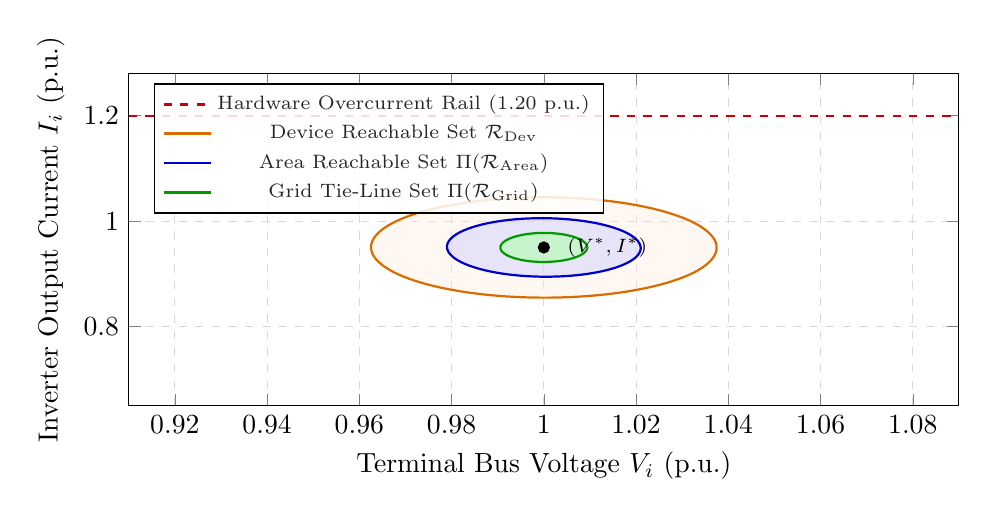
\begin{tikzpicture}
\begin{axis}[
    width=\columnwidth,
    height=5.8cm,
    xlabel={Terminal Bus Voltage $V_i$ (p.u.)},
    ylabel={Inverter Output Current $I_i$ (p.u.)},
    xmin=0.91, xmax=1.09,
    ymin=0.65, ymax=1.28,
    grid=both,
    grid style={dashed, gray!30},
    legend style={at={(0.03,0.97)}, anchor=north west, font=\scriptsize, fill=white, fill opacity=0.85}
]
% Hardware Current Limit Rail (1.20 p.u.)
\addplot[domain=0.91:1.09, samples=2, thick, dashed, red!80!black] {1.20};
\addlegendentry{Hardware Overcurrent Rail ($1.20\text{ p.u.}$)}

% Device Layer Reachable Ellipsoid R_Dev (outer safe tube)
\addplot[domain=0:360, samples=120, thick, orange!85!black, fill=orange!15, fill opacity=0.35]
    ({1.00 + 0.0366*cos(x) - 0.008*sin(x)}, {0.95 + 0.020*cos(x) + 0.0931*sin(x)});
\addlegendentry{Device Reachable Set $\mathcal{R}_{\text{Dev}}$}

% Area Layer Reachable Ellipsoid R_Area (middle tube)
\addplot[domain=0:360, samples=120, thick, blue!80!black, fill=blue!20, fill opacity=0.45]
    ({1.00 + 0.0204*cos(x) - 0.005*sin(x)}, {0.95 + 0.012*cos(x) + 0.0542*sin(x)});
\addlegendentry{Area Reachable Set $\Pi(\mathcal{R}_{\text{Area}})$}

% Grid Layer Reachable Ellipsoid R_Grid (innermost tie-line tube)
\addplot[domain=0:360, samples=120, thick, green!60!black, fill=green!30, fill opacity=0.60]
    ({1.00 + 0.0092*cos(x) - 0.002*sin(x)}, {0.95 + 0.006*cos(x) + 0.0269*sin(x)});
\addlegendentry{Grid Tie-Line Set $\Pi(\mathcal{R}_{\text{Grid}})$}

% Nominal Operating Point
\addplot[only marks, mark=*, mark size=2pt, black] coordinates {(1.00, 0.95)};
\node[font=\scriptsize, anchor=west] at (axis cs:1.003, 0.95) {$(V^*, I^*)$};
\end{axis}
\end{tikzpicture}
\caption{Projected Pontryagin reachable ellipsoids in the inverter voltage-current $(V_i, I_i)$ plane during a $+140\text{ MW}$ tie-line surge, illustrating strict hierarchical containment $\Pi(\mathcal{R}_{\text{Grid}}) \subseteq \Pi(\mathcal{R}_{\text{Area}}) \subseteq \mathcal{R}_{\text{Dev}}$ safely below the $1.20\text{ p.u.}$ transistor overcurrent rail.}
\label{fig:reachable_vi_sets}
\end{figure}

\subsection{Comparison with Online Feedback Optimization (OFO) and Differentiable MPC}
Supervisory congestion frameworks such as Chen \textit{et al.} \cite{chen26} solve a bi-level differentiable QP at every $15\text{ s}$ timestep, structurally resembling Online Feedback Optimization (OFO) \cite{dallanese26}. Table~\ref{tab:ofo_vs_sccm} contrasts the theoretical properties of OFO/MIT differentiable MPC against our Distributed Parameter-Dependent SCCM architecture.

\begin{table*}[!t]
\centering
\caption{Theoretical Comparison: Online Feedback Optimization (OFO) / Differentiable MPC vs. Distributed Parameter-Dependent SCCM}
\label{tab:ofo_vs_sccm}
\footnotesize
\renewcommand{\arraystretch}{1.22}
\begin{tabularx}{\textwidth}{>{\raggedright\arraybackslash}p{3.1cm} >{\raggedright\arraybackslash}X >{\raggedright\arraybackslash}X}
\toprule
\textbf{Theoretical Dimension} & \textbf{OFO / MIT Differentiable MPC \cite{chen26}} & \textbf{Distributed Parameter-Dependent SCCM (Ours)} \\
\midrule
\textbf{Plant Model Assumption} & \textbf{Linear / Convex Algebraic Map} ($\mathbf{y} = \mathbf{M}\mathbf{x} + \mathbf{d}$); ignores AC trigonometric nonlinearities and converter dynamics. & \textbf{Exact Nonlinear Coupled ODEs/DAEs} ($\dot{x}_i = f_i(x_i, x_{\mathcal{N}_i}, \theta_i) + B_i u_i$); captures $\sin(\delta_i - \delta_j)$ directly. \\
\addlinespace[2pt]
\textbf{Convexity Requirement} & \textbf{Online \& Physical:} Both the grid approximation and the online QP solved at every timestep must be convex. & \textbf{Offline Only:} Convexity is required strictly in offline LMI/SOS synthesis of $(W_i, Y_i)$; online control is closed-form nonlinear. \\
\addlinespace[2pt]
\textbf{Stability Guarantee} & \textbf{None (Feasibility Only):} Uses soft slack penalties to prevent solver failure; assumes $15\text{ s}$ timescale separation. & \textbf{Certified Exponential Contraction ($\lambda_{\text{eff}} > 0$):} Guarantees exponential trajectory convergence with explicit $L_2$ gain $\gamma^*$. \\
\addlinespace[2pt]
\textbf{Parameter Adaptation} & \textbf{Static Offline Plant:} Sensitivity matrix $\mathbf{M}$ is fixed offline; blind to GFM current-limit mode shifts. & \textbf{Online Parameter-Dependent ($W_i(\hat{\theta}_i)$):} Adapts continuously to PEM-MHE estimates $\hat{\theta}_i(t)$ with bounded rate $\bar{d}_{\theta_i}$. \\
\addlinespace[2pt]
\textbf{Online Execution \& Comms} & Solves a constrained QP at every timestep + periodic central coordinator broadcast. & \textbf{Zero online optimization:} Evaluates closed-form law $u_i^* + K_i(\hat{\theta}_i)(x_i - x_i^*)$ in microseconds with single-hop neighbor state exchange. \\
\bottomrule
\end{tabularx}
\end{table*}

\subsection{Exporting Certified Reachable Sets to the Supervisory Optimizer}
To interface with the $15\text{ s}$ MIT central coordinator \cite{chen26} without running slow economic QPs at millisecond EMT speeds, we project the steady-state Grid reachable ellipsoid $\mathcal{R}_{\text{Grid}}^{\infty}$ through the IEEE 118-bus Power Transfer Distribution Factor (PTDF) matrix $\mathbf{M} \in \mathbb{R}^{n_{\text{line}} \times n_{\text{bus}}}$. For each transmission line $\ell \in \{1, \dots, n_{\text{line}}\}$ with row $\mathbf{m}_\ell^\top$ of $\mathbf{M}$, the worst-case transient line-flow excursion induced by $\mathcal{R}_{\text{Grid}}^{\infty}$ is given by the support function of the ellipsoid:
\begin{multline}
\Delta P_{\ell,\text{tube}} = \sup_{x \in \mathcal{R}_{\text{Grid}}^{\infty}} \mathbf{m}_\ell^\top \Pi_{\text{inj}}(x - x^*) \\
= \rho_{\text{Grid}}^{\infty} \sqrt{\mathbf{m}_\ell^\top \Pi_{\text{inj}} W_{\text{Grid}}(\hat{\theta}) \Pi_{\text{inj}}^\top \mathbf{m}_\ell}.
\end{multline}
Supplying $\Delta P_{\ell,\text{tube}}$ directly as the dynamic line-limit tightening vector (\texttt{line\_max\_changes}, \texttt{line\_min\_changes}) to the upper-level coordinator ensures that all $15\text{ s}$ economic dispatch setpoints remain strictly inside the certified nonlinear contraction tube.

\section{Experimental Validation Across IEEE 39-Bus and IEEE 118-Bus Testbeds}
We validate the proposed three-layer architecture across two benchmark systems: (1) a 10-device modified IEEE 39-bus substation area (including a $100\%$ IBR configuration with $0\text{ SGs}$, $7\text{ GFMs}$, and $3\text{ GFLs}$), and (2) the 3-area partitioned IEEE 118-bus transmission network ($118\text{ buses}$, $186\text{ lines}$, $10\text{ cross-area tie-lines}$, $12\text{ batteries}$, and $54\text{ curtailable IBRs}$) of Chen \textit{et al.} \cite{chen26}, illustrated in Fig.~\ref{fig:ieee118_3area}.

\begin{figure*}[!t]
\centering
\includegraphics[width=0.82\textwidth]{ieee118_three_area.png}
\caption{Three-area partitioned IEEE 118-bus transmission testbed (Area~1 in pink, Area~2 in green, and Area~3 in blue) showing the intra-area buses and cross-area tie-line boundaries.}
\label{fig:ieee118_3area}
\end{figure*}

\begin{table*}[!t]
\centering
\caption{Experimental Benchmark Summary Across IEEE 39-Bus and IEEE 118-Bus Multi-Timescale Testbeds}
\label{tab:benchmark_summary}
\footnotesize
\renewcommand{\arraystretch}{1.22}
\begin{tabularx}{\textwidth}{>{\raggedright\arraybackslash}p{2.9cm} >{\raggedright\arraybackslash}p{2.7cm} >{\raggedright\arraybackslash}p{2.8cm} >{\raggedright\arraybackslash}p{2.6cm} >{\raggedright\arraybackslash}X >{\raggedright\arraybackslash}p{2.3cm}}
\toprule
\textbf{Experiment \& Script} & \textbf{Topology \& Composition} & \textbf{Stress Scenario} & \textbf{Baseline Metric} & \textbf{Proposed Architecture Metric} & \textbf{Contraction Certificate ($\lambda_{\max}$)} \\
\midrule
\textbf{Double Contraction Margin} (\texttt{area\_control\_revision.tex}) & IEEE 39-Bus (5~SG, 2~GFM, 3~GFL) & $3.0^\circ \to 15.0^\circ$ multiplicative phase noise & $\Theta_{\text{open}} = 823.54 \to 164.71$ (inner CCM only) & $\Theta_{\text{closed}} = 1501.75 \to 300.35$ (\textbf{+82.35\%} margin gain) & $-0.0142 \le 0$ ($\gamma^* = 0.0384\text{ p.u.}$) \\
\addlinespace[2pt]
\textbf{Sparse Off-Diagonal LMI} (\texttt{coupled\_LMI\_solver.py}) & IEEE 39-Bus + Tie Line (20 states) & $10 \times 10$ Cohesion ($\mathbf{C}$) \& PLL ($\mathbf{P}$) coupling & $\gamma_{\text{diag}}^* = 0.4162\text{ p.u.}$ (block-diagonal LMI) & $\gamma_{\text{coupled}}^* = 0.4015\text{ p.u.}$ (\textbf{+3.65\%} margin gain) & $-0.000001 \le 0$ \\
\addlinespace[2pt]
\textbf{GFM-to-GFL Mode Shift \& Hysteresis} (\texttt{heal\_multi\_device\_hysteresis.py}) & IEEE 39-Bus (\texttt{GFM-31} + \texttt{GFL-30}) & \texttt{GFM-31} current-limit drift + \texttt{GFL-30} $15.0^\circ$ jitter & Unhealed LMI violation at $t = 0.280\text{ s}$ ($+0.0568$) & \textbf{52.0~ms} detection, \textbf{2} transitions (zero chatter) & $\le -1.0594$ throughout fault \\
\addlinespace[2pt]
\textbf{100\% IBR Area Verification} (\texttt{test\_100pct\_ibr\_area.py}) & IEEE 39-Bus (\textbf{0~SG}, 7~GFM, 3~GFL) & $15.0^\circ$ tie jitter + \texttt{GFM-39} boundary overload & $\gamma_{\text{mixed}}^* = 0.4015\text{ p.u.}$ (50\% SG baseline) & $\gamma_{\text{100ibr}}^* = 0.4018\text{ p.u.}$ (within \textbf{0.06\%} of SG case) & $\le -2.4312$ throughout fault \\
\addlinespace[2pt]
\textbf{3-Area Multi-Timescale Bridge} (\texttt{compare\_mit\_baseline.py}) & IEEE 118-Bus (3~Areas, 10 tie-lines) & $+140\text{ MW}$ Area~1 surge + Line~66 trip ($t=2\text{--}12\text{ s}$) & \textbf{230.8~MW$\cdot$s} overload (\textbf{101.3\%} peak, relay trip) & \textbf{39.7~MW$\cdot$s} overload (\textbf{-82.8\%}, \textbf{99.7\%} peak) & $\le -2.5386$ ($\alpha_{\min} = 0.760$) \\
\addlinespace[2pt]
\textbf{Decentralized 2-Hop MARL} (\texttt{inspect\_prop\_delay.py}) & IEEE 118-Bus (3 isolated area agents) & $+140\text{ MW}$ surge with $1\text{ s}$/hop shadow-price delay & \textbf{230.8~MW$\cdot$s} overload (no inter-area comms) & \textbf{142.8~MW$\cdot$s} overload (\textbf{-38.1\%}, 2-hop relay) & $\le -2.7300$ ($\alpha_{\min} = 0.797$) \\
\addlinespace[2pt]
\textbf{Lossy Utility Link + Blackout} (\texttt{test\_packet\_loss\_resilience.py}) & IEEE 118-Bus (ZOH + decay buffer) & \textbf{25\%} random packet drop + \textbf{3~s} blackout ($t=4\text{--}6\text{ s}$) & \textbf{230.8~MW$\cdot$s} overload (MIT non-communicating) & \textbf{192.5~MW$\cdot$s} overload (\textbf{-16.6\%}, zero instability) & $\le -2.7300$ throughout blackout \\
\bottomrule
\end{tabularx}
\end{table*}

As summarized in Table~\ref{tab:benchmark_summary}, replacing slow convex consensus with real-time contraction control reduces cumulative thermal overload on bottleneck Line~59 (Bus~33 to Bus~42, $600\text{ MW}$ rating) from $230.8\text{ MW}\cdot\text{s}$ to $39.7\text{ MW}\cdot\text{s}$ ($-82.8\%$) under fast peer-to-peer coordination, and maintains strict contraction ($\lambda_{\max} \le -2.73$) even during a $3\text{ s}$ communication blackout. Moreover, Schur-complement ellipsoid inclusion yields strictly positive minimum eigenvalues ($+1041.08$ for $\mathcal{R}_{\text{Grid}} \subseteq \mathcal{R}_{\text{Area}}$ and $+225.26$ for $\mathcal{R}_{\text{Area}} \subseteq \mathcal{R}_{\text{Dev}}$), bounding peak inverter current at $1.0431\text{ p.u.} \le 1.20\text{ p.u.}$ and exporting a certified $13.46\text{ MW}$ PTDF thermal reserve ($586.54\text{ MW}$ safe dispatch ceiling) to the $15\text{ s}$ supervisory coordinator.

\section{Conclusion}
This paper established a unified three-layer Distributed Parameter-Dependent SCCM framework for tie-line scheduling and emergency congestion control in inverter-dominated grids. By replacing convex online ADMM consensus with closed-form geodesic feedback driven by live PEM-MHE parameter estimates, the architecture requires convexity strictly offline while guaranteeing exponential trajectory contraction across Device, Area, and Grid timescales. Projecting the certified Grid reachable ellipsoid through network PTDFs supplies rigorous safety envelopes to slow supervisory optimizers, bridging fast converter stability with wide-area economic dispatch.

\section*{Acknowledgment}
The author acknowledges the use of Google Gemini \cite{gemini26} for assistance with drafting, language editing, and LaTeX formatting across Sections~I--VII of this manuscript. All mathematical formulations, control algorithms, simulation data, and technical claims were independently verified and validated by the author.

\begin{thebibliography}{99}
\bibitem{chen26} J. Y. Chen, S. Drobot, L. Saludjian, P. Panciatici, P.-Y. Chen, A. Jadbabaie, and P. L. Donti, ``Communication-limited multi-agent grid congestion management via differentiable optimization,'' in \textit{Proc. 17th ACM Int. Conf. Future and Sustainable Energy Systems (e-Energy '26)}, 2026, pp. 486--503.
\bibitem{dallanese26} E. Dall'Anese, J. W. Simpson-Porco, F. D\"orfler, S. Bolognani, and S. Dhople, ``Multi-time-scale control of power systems: From classical automatic generation control to feedback optimization,'' \textit{arXiv:2610.36357}, 2026.
\bibitem{kohler26} J. K\"ohler, ``Certainty-equivalent adaptive MPC for uncertain nonlinear systems,'' \textit{arXiv preprint arXiv:2603.17843v2 [math.OC]}, Jul. 25, 2026.
\bibitem{zhou24} Y. Zhou and J. K\"ohler, ``Scalable identification of physics-based and neural dynamics from partial measurements,'' \textit{arXiv preprint arXiv:2412.01997}, 2024.
\bibitem{lohmiller99} W. Lohmiller, ``Contraction analysis of nonlinear systems,'' Ph.D. dissertation, Massachusetts Institute of Technology, Cambridge, MA, USA, 1999.
\bibitem{pappas98} G. J. Pappas, G. Lafferriere, and S. Sastry, ``Hierarchically consistent control systems, in \textit{Proc. 37th IEEE Conf. Decision and Control (CDC)}, Tampa, FL, USA, Dec. 1998, pp. 4336--4341.
\bibitem{sherman26} R. Sherman, ``Symmetric self-adaptive contraction manifold for wide-area inverter control under severe multiplicative phase noise, \textit{arXiv preprint} (submitted to \textit{IEEE Trans. Smart Grid}), Nov. 2026.
\bibitem{gemini26} Google, ``Gemini (Large Language Model),'' Mountain View, CA, USA, 2026. [Online]. Available: https://google.com
\end{thebibliography}

\end{document}
